\section{A Key-Only Universal Forgery}\label{sec:keyonly}

The paper's attacker is strong: a malicious KGC that holds the master key and the victim's certificate and
has observed one signature. We asked whether a much weaker attacker suffices.

\subsection{The forgery}
\prov{Ours}. Consider Verma's verification equation for a single signature,
\begin{equation}\label{eq:verma-single}
zP=R+h_0\PTA+v\,pk,\qquad h_0=H_0(id\concat pk),\qquad v=H_1(m\concat pk\concat id\concat\Delta).
\end{equation}
Neither hash contains $R$, $R$ appears with coefficient 1, and $R$ travels inside the signature, so the
signer (or a forger) chooses it.

\begin{proposition}[Key-only universal forgery]\label{prop:keyonly}
Let $id$ and $pk$ belong to an honestly enrolled signer of Verma's scheme, as specified in Section~IV-A
of~\cite{qiao2023}. Given only the public values $\PTA$, $id$, $pk$ and $\Delta$, an adversary can output,
for any message $m$, a pair $(R,z)$ that the verification equation \eqref{eq:verma-single} accepts. It
succeeds with probability 1, sees no signature, and computes no discrete logarithm.
\end{proposition}

\begin{proof}
The adversary (1) picks any $z\in\Zp$, for example $z=0$; (2) computes $h_0=H_0(id\concat pk)$ and
$v=H_1(m\concat pk\concat id\concat\Delta)$, whose inputs are all public; and (3) sets
$R=zP-h_0\PTA-v\,pk$. The verifier recomputes the same $h_0$ and $v$, because neither depends on $R$, and
\[
R+h_0\PTA+v\,pk=(zP-h_0\PTA-v\,pk)+h_0\PTA+v\,pk=zP,
\]
so \eqref{eq:verma-single} holds. No step can fail, so the probability is 1, and the cost is two hashes,
three scalar multiplications and two point subtractions.
\end{proof}

The forgery uses only point arithmetic: no
secret, no observed signature, no interaction with the KGC or the victim, and no discrete logarithm. In
the taxonomy of~\cite{gmr1988} it is a key-only universal forgery, the strongest kind. It is the familiar
failure of a Schnorr signature whose challenge omits the commitment, $c=H(m)$ instead of
$c=H(R,m)$~\cite{schnorr1991}. We have not found it discussed for Verma's scheme, but we did not survey
the literature exhaustively, so we claim only that the paper does not discuss it.

\paragraph{Results.} Against a real, honestly enrolled victim key, the forgery verifies in 8 of 8 trials
(4 messages $\times$ 2 backends), and 8 of 8 forgeries also pass aggregate verification next to an honest
signature. \Cref{fig:keyonly} shows the captured output of the demonstration.

\begin{figure}[ht]
\centering
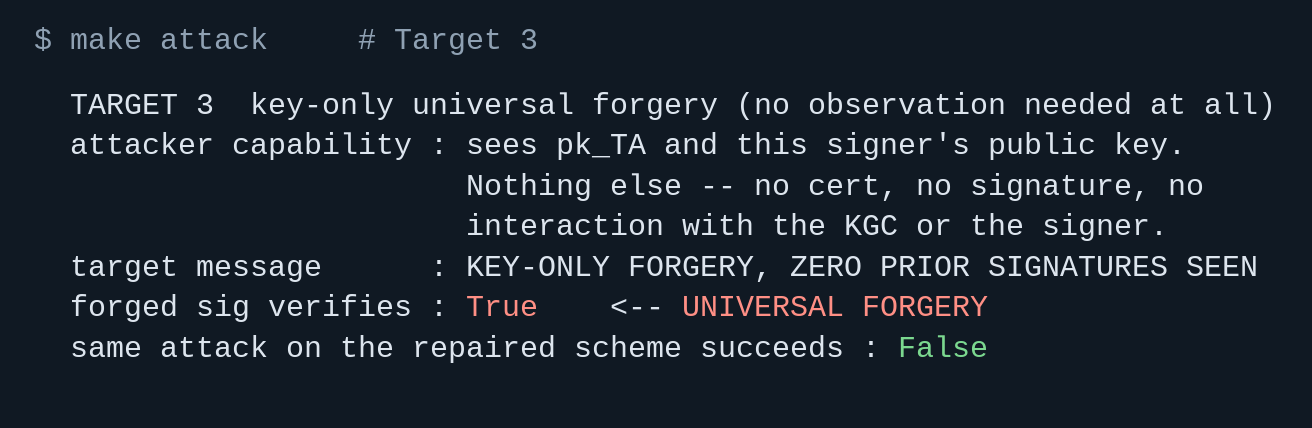
\includegraphics[width=0.9\linewidth]{figures/final_demo1_keyonly.png}
\caption{Captured output of \code{make attack}, Target~3: a forgery from the victim's public key alone
verifies; the same attack on the repaired scheme does not.}\label{fig:keyonly}
\end{figure}

\subsection{It contradicts the paper's Table II}
Table~II of the paper rates Verma's scheme (its reference~[11]) as \emph{secure} against $\Fone$, the
malicious user, and insecure against $\Ftwo$, the malicious KGC~\cite{qiao2023}. The $\Ftwo$ entry is the
paper's own attack (\cref{sec:repro}). The $\Fone$ entry cannot be right: our forger has strictly less
power than $\Fone$, which may additionally replace keys and obtain signatures, so whatever it achieves
$\Fone$ achieves too. This holds for Verma's scheme as the paper specifies it in its Section~IV-A, which
is the scheme the paper's table rates; we did not check Verma's original article~\cite{verma2020}.

\subsection{Why the repaired scheme resists it}
In the repaired equation \eqref{eq:qiao-verify}, $R$ enters all three hashes and $T$ enters two. To solve
for $R$ an attacker needs $h_0$, $u$ and $v$; to compute them it needs $R$. The only route left is a
search for a fixed point of the hash functions: guess $R$, compute the hashes, solve for the $R$ the
equation would require, and compare. In every trial 16 rounds of this search produced 16 distinct
candidates and no forgery. This shows the attack does not apply; it is not a proof of security, which is
the role of the paper's theorem.

\subsection{Which binding closes which door}
The repair binds two commitments at once: $T$ (the signature's nonce commitment) and $R$ (the certificate
commitment). We removed each in turn, keeping everything else, and attacked each variant both by solving
for $T$ and by solving for $R$ (\cref{tab:2x2}).

\begin{table}[ht]
\centering\small
\caption{The $2\times2$ ablation. Each cell reports which attack succeeds (8/8 trials per cell).}
\label{tab:2x2}
\begin{tabularx}{\linewidth}{lXX}
\toprule
& $R$ hashed & $R$ not hashed \\
\midrule
$T$ hashed & \textbf{Repaired scheme}: both attempts fail &
  \textbf{$R$ removed}: solving for $R$ forges, but only under an attacker-chosen $R$ (public-key replacement) \\
$T$ not hashed & \textbf{$T$ removed}: solving for $T$ forges with the victim's real certificate (key-only) &
  \textbf{Verma}: solving for $R$ forges; $R$ travels in the signature (key-only) \\
\bottomrule
\end{tabularx}
\end{table}

In each broken variant the other attempt still fails (8/8), so each binding blocks a different attack
and neither covers for the other. The two open doors differ in kind. $T$ travels in every signature, so
the $T$-removed forgery is a key-only forgery against the real public key. In the repaired scheme, by
contrast, $R$ belongs to the certificate, so the $R$-removed forgery verifies only if the verifier
accepts an attacker-chosen $R$; under the real certificate value it fails in 8 of 8 trials. That is
public-key replacement, the power the paper grants $\Fone$, and it is exactly the reason the paper gives
for hashing $R$. The cell thus confirms the paper's stated rationale with code.

\paragraph{The general rule.} Any value that appears in the verification equation with a known
coefficient but in no hash is a free variable, and an attacker can fix everything else and solve for it.
The paper states this rule for $T_i$ alone, in the context of its one attack; the $2\times2$ shows the
same mechanism for either commitment independently.
